\documentclass[]{article}
\usepackage{lmodern}
\usepackage{amssymb,amsmath}
\usepackage{ifxetex,ifluatex}
\usepackage{fixltx2e} % provides \textsubscript
\ifnum 0\ifxetex 1\fi\ifluatex 1\fi=0 % if pdftex
  \usepackage[T1]{fontenc}
  \usepackage[utf8]{inputenc}
\else % if luatex or xelatex
  \ifxetex
    \usepackage{mathspec}
  \else
    \usepackage{fontspec}
  \fi
  \defaultfontfeatures{Ligatures=TeX,Scale=MatchLowercase}
\fi
% use upquote if available, for straight quotes in verbatim environments
\IfFileExists{upquote.sty}{\usepackage{upquote}}{}
% use microtype if available
\IfFileExists{microtype.sty}{%
\usepackage{microtype}
\UseMicrotypeSet[protrusion]{basicmath} % disable protrusion for tt fonts
}{}
\usepackage[margin=1in]{geometry}
\usepackage{hyperref}
\hypersetup{unicode=true,
            pdftitle={Individual differences in visual perception in adults},
            pdfauthor={Rick Gilmore, Yiming Qian, \& Andrea Seisler},
            pdfborder={0 0 0},
            breaklinks=true}
\urlstyle{same}  % don't use monospace font for urls
\usepackage{longtable,booktabs}
\usepackage{graphicx,grffile}
\makeatletter
\def\maxwidth{\ifdim\Gin@nat@width>\linewidth\linewidth\else\Gin@nat@width\fi}
\def\maxheight{\ifdim\Gin@nat@height>\textheight\textheight\else\Gin@nat@height\fi}
\makeatother
% Scale images if necessary, so that they will not overflow the page
% margins by default, and it is still possible to overwrite the defaults
% using explicit options in \includegraphics[width, height, ...]{}
\setkeys{Gin}{width=\maxwidth,height=\maxheight,keepaspectratio}
\IfFileExists{parskip.sty}{%
\usepackage{parskip}
}{% else
\setlength{\parindent}{0pt}
\setlength{\parskip}{6pt plus 2pt minus 1pt}
}
\setlength{\emergencystretch}{3em}  % prevent overfull lines
\providecommand{\tightlist}{%
  \setlength{\itemsep}{0pt}\setlength{\parskip}{0pt}}
\setcounter{secnumdepth}{0}
% Redefines (sub)paragraphs to behave more like sections
\ifx\paragraph\undefined\else
\let\oldparagraph\paragraph
\renewcommand{\paragraph}[1]{\oldparagraph{#1}\mbox{}}
\fi
\ifx\subparagraph\undefined\else
\let\oldsubparagraph\subparagraph
\renewcommand{\subparagraph}[1]{\oldsubparagraph{#1}\mbox{}}
\fi

%%% Use protect on footnotes to avoid problems with footnotes in titles
\let\rmarkdownfootnote\footnote%
\def\footnote{\protect\rmarkdownfootnote}

%%% Change title format to be more compact
\usepackage{titling}

% Create subtitle command for use in maketitle
\providecommand{\subtitle}[1]{
  \posttitle{
    \begin{center}\large#1\end{center}
    }
}

\setlength{\droptitle}{-2em}

  \title{Individual differences in visual perception in adults}
    \pretitle{\vspace{\droptitle}\centering\huge}
  \posttitle{\par}
    \author{Rick Gilmore, Yiming Qian, \& Andrea Seisler}
    \preauthor{\centering\large\emph}
  \postauthor{\par}
      \predate{\centering\large\emph}
  \postdate{\par}
    \date{2019-11-13 15:06:43}


\begin{document}
\maketitle

{
\setcounter{tocdepth}{3}
\tableofcontents
}
\section{Purpose}\label{purpose}

This document serves as the master protocol for the study.

\section{Key references}\label{key-references}

Abramov, I., Gordon, J., Feldman, O., \& Chavarga, A. (2012). Sex \&
vision I: Spatio-temporal resolution. \emph{Biology of Sex Differences},
\emph{3}(1), 20. Retrieved from
\url{http://dx.doi.org/10.1186/2042-6410-3-20}

Murray, S. O., Schallmo, M.-P., Kolodny, T., Millin, R., Kale, A.,
Thomas, P., Rammsayer, T. H., et al. (2018). Sex differences in visual
motion processing. \emph{Current Biology}. Retrieved from
\url{http://dx.doi.org/10.1016/j.cub.2018.06.014}

\section{IRB}\label{irb}

This protocol, ``Individual differences in visual perception in
adults,'' has been assigned protocol number 13345. The most recent IRB
approval was granted on 2010-10-14. Files related to the approved
(exempt) submission can be found \href{../irb/2019-10-24}{here}. Minor
modifications of the items in the forms do not need to submit a
modification.

\section{Prior to data collection
start}\label{prior-to-data-collection-start}

\subsection{Equipment preparation}\label{equipment-preparation}

First, we need to do benchmark testing to determine what screen
resolution will work at the highest temporal resolution (120 Hz). This
study requires high temporal resolution in order to measure temporal
thresholds--the shortest stimulus duration that participants require in
order to accurately detect the direction of motion. Replication of
Abramov et al. (2012) study requires the best luminance resolution,
which permitted the presentation of very low contrast stimuli. Once we
have determined the best monitor settings, we will calibrate the monitor
before we start collecting data. Those steps follow.

\subsection{Calibrate Monitor}\label{calibrate-monitor}

\subsubsection{Prepare Computers}\label{prepare-computers}

\begin{itemize}
\tightlist
\item
  In 503B Switch on power of large surge protector on bottom left shelf.
\end{itemize}

\subsubsection{Prepare Photometer}\label{prepare-photometer}

\begin{itemize}
\tightlist
\item
  Take the photometer out of the box.
\item
  Set it up by plugging in the power and the light meter.
\item
  Turn on the photometer
\item
  Ensure the following settings:
\item
  Zero the photometer by placing the cap on the light meter and pressing
  the `zero' button
\end{itemize}

\subsubsection{Start Calibrating
Luminance}\label{start-calibrating-luminance}

\begin{itemize}
\item
  Turn on the computer
\item
  In 503B switch on power of large surge protector on bottom left shelf.
\item
  Log-in (Gilmore Lab)
\item
  Start Psychopy - Click icon on Task Bar
\item
  Open Monitor Settings - Go to Tools \textgreater{} Monitor Center
\item
  Click \textbf{XXXX}
\item
  Enter the Monitor Screen Width in centimeters
\item
  Select \textbf{Start}\\
\end{itemize}

We may check the monitor calibration during data collection at a
frequency we will decide later.

\subsection{Survey preparation}\label{survey-preparation}

This study uses Qualtrics to collect implied/oral consent and other data
from participants. Yiming has generated a draft survey, saved
\href{qualtrics_survey.qsf}{here} as a \texttt{*.qsf} format text file.

The URL for the survey is
\url{https://pennstate.qualtrics.com/jfe/form/SV_0Cad5AtrbQN0GKV}

\section{Scheduling participants}\label{scheduling-participants}

\subsection{Overview}\label{overview}

Rick Gilmore is the PI on the SONA Systems study (Study ID 2587)
associated with this protocol. Yiming Qian and Andrea Seisler are
researchers. The URL is
\url{https://pennstate.sona-systems.com/exp_info.aspx?experiment_id=2587}.

The process of scheduling participants involves the following steps:

\begin{enumerate}
\def\labelenumi{\arabic{enumi}.}
\tightlist
\item
  Create slots on SONA with specific dates and times
\item
  When slot is scheduled, email sent to Yiming and Andrea in the system.
\item
  Scheduled slots will be added to lab calendar.
\end{enumerate}

\begin{itemize}
\tightlist
\item
  The scheduled RA will be added to the title of the slot
\item
  The RA will also be invited to the google calendar event.
\end{itemize}

\begin{enumerate}
\def\labelenumi{\arabic{enumi}.}
\setcounter{enumi}{3}
\tightlist
\item
  Researchers will be contacted by email and Discord by Yiming or Andrea
  if they are needed for a slot that is not part of their regularly
  scheduled lab time.
\end{enumerate}

\subsection{Weekly testing slots}\label{weekly-testing-slots}

\begin{longtable}[]{@{}llll@{}}
\toprule
Day of Week & Time & Researcher(s) & Lead\tabularnewline
\midrule
\endhead
Mon & 09:00a & Rachel & Andrea\tabularnewline
& 10:15a & Sandy, Emily, Rachel & Andrea\tabularnewline
& 11:30a & Sandy, Emily, Amar & Yiming\tabularnewline
& 1p & Emily & Yiming\tabularnewline
& 2:15p & & Yiming\tabularnewline
& 3:30p & & Yiming\tabularnewline
& 4:45p & & Yiming\tabularnewline
Tue & 09:00a & Michelle, Rachel & Andrea\tabularnewline
& 10:15a & Michelle, Rachel & Andrea\tabularnewline
& 11:30a & Amar, Michelle & Andrea\tabularnewline
& 12:45p & Michelle, Joseph, Amar & Andrea\tabularnewline
Wed & 10:00a & Sandy, Rachel, Amar & Yiming\tabularnewline
& 11:15a & Sandy, Rachel, Amar, Emily & Andrea\tabularnewline
& 12:30p & Luka, Emily & Andrea\tabularnewline
& 01:45p & & Yiming\tabularnewline
& 03:00p & & Yiming\tabularnewline
& 04:15p & & Yiming\tabularnewline
& 05:30p & & Yiming\tabularnewline
Thu & 09:00a & Joseph, Michelle, Luka,Rachel & Yiming\tabularnewline
& 10:15 & Rachel & Yiming\tabularnewline
& 11:30a & Amar &\tabularnewline
& 01:30p & Luka & Yiming (every two weeks)\tabularnewline
& 02:45p & & Yiming (every two weeks)\tabularnewline
& 04:00p & & Yiming\tabularnewline
& 05:15p & Emily & Yiming\tabularnewline
Fri & 09:00a & Rachel & Yiming\tabularnewline
& 10:15a & Rachel, Emily, Amar & Yiming\tabularnewline
& 11:30a & Rachel, Emily, Amar & Andrea\tabularnewline
& 12:45p & Emily, Amar & Andrea\tabularnewline
& 02:00p & Michelle & Yiming\tabularnewline
& 03:15p & & Yiming\tabularnewline
& 04:30p & & Yiming\tabularnewline
\bottomrule
\end{longtable}

\section{Day of visit}\label{day-of-visit}

\subsection{Before participant
arrives}\label{before-participant-arrives}

\begin{itemize}
\tightlist
\item
  Check to see if there have been any cancellations.
\item
  If the scheduled study is still on the books, proceed as follows.
\end{itemize}

\subsubsection{Set-up for Vision
Screening}\label{set-up-for-vision-screening}

\paragraph{Preparation}\label{preparation}

Materials for vision screening are stored on the table next to Andrea's
office.

\begin{itemize}
\tightlist
\item
  Make sure the black tape is on the floor 10ft from the HOVT Snellen
  Acuity Chart which is on the door to 503B
\item
  Place Stereo Acuity Test and Glasses on table
\item
  Place Color Vision Test on table
\item
  Place the Vision Screening Score Sheet on the table
\end{itemize}

\paragraph{Review vision screening
procedures}\label{review-vision-screening-procedures}

The vision screening protocol may be reviewed at
\href{vision-screening-protocol.html}{this link}

\subsubsection{Set up for computer-based
tasks}\label{set-up-for-computer-based-tasks}

\paragraph{Stimuli Computer}\label{stimuli-computer}

\begin{itemize}
\item
  \emph{Log into Data Collection Computer}
\item
  Turn on the power of the data collection computer
\item
  Turn on the CRT monitor in 503B
\item
  Log-in (Gilmore Lab)
\item
  \emph{Start Psychopy}
\item
  Click \textbf{PsychoPy} icon on Task Bar
  
\includegraphics{images/PsychoPy-1.PNG}\\
\item
  \emph{Double-check monitor settings within Windows}
\item
  Click Settings (`gear') icon on Task Bar
  
\includegraphics{images/DispSettings-1.PNG}\\
\item
  Choose \textbf{System}\\
  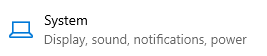
\includegraphics{images/DS2.PNG}\\
\item
  Choose \textbf{Display}\\
  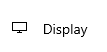
\includegraphics{images/ds3.PNG}\\
\item
  Choose \textbf{Advanced display settings} (You may need to scroll down
  to see this)\\
  
\includegraphics{images/DS4.PNG}\\
\item
  Make sure the window that appears has the following Settings\\
  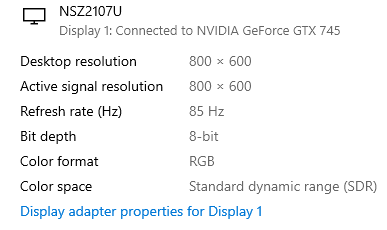
\includegraphics{images/ds5.PNG}\\
\item
  \emph{Double-check Brightness/Contrast of monitor}
\item
  Contrast:
\item
  Brightness:
\item
  Press any button on the monitor (except Signal A/B/OSD OFF and the
  Power button)
\item
  Navigate to the leftmost option in the settings menu (looks like a
  half moon)
\item
  Press the down button on the monitor
\item
  Adjust the Contrast (leftmost option) to the required setting using
  the +/- buttons on the monitor
\item
  Adjust the Brightness (second option from the left) to the required
  setting using the +/- buttons on the monitor
\item
  \emph{Check monitor within PsychoPy}\\
\item
  Go to \textbf{Monitor Settings}\\
  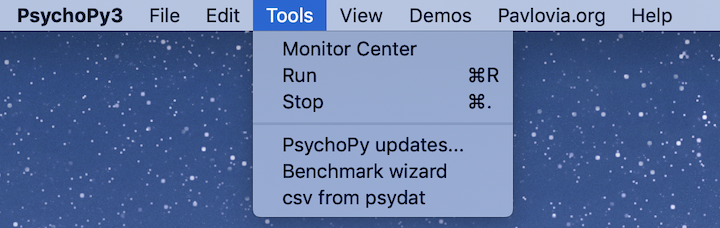
\includegraphics{images/pp2.png}\\
\item
  View Settings, they should be as follows\\
  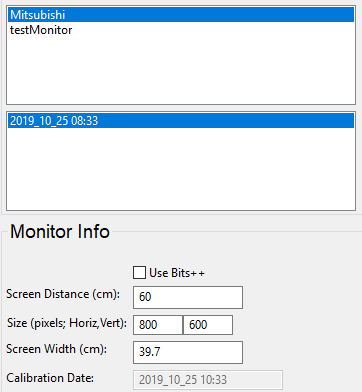
\includegraphics{images/pp3.PNG}
\end{itemize}

\paragraph{Survey Computer}\label{survey-computer}

\begin{itemize}
\tightlist
\item
  Log-in to survey computer
\item
  Load page with surveys:
  \url{https://pennstate.qualtrics.com/jfe/form/SV_0Cad5AtrbQN0GKV}
\end{itemize}

\subsubsection{After participant
arrives}\label{after-participant-arrives}

\paragraph{Welcome participant}\label{welcome-participant}

Say:

\begin{quote}
``\emph{Welcome to the brain, behavior, and development lab. Are you
here for the study about individual difference of motion perception?}''
\end{quote}

Close the door. If the participant answers yes, say:

\begin{quote}
``\emph{Great. You can sit in this chair and put your coat and bags
beside you.}''
\end{quote}

\begin{itemize}
\tightlist
\item
  Store coat on back of main door and bags by the file/bookcase.
\end{itemize}

\begin{quote}
``\emph{Are you \textless{}NAME OF PERSON ON SONA SYSTEMS SITE SCHEDULED
FOR THIS SESSION\textgreater{}?}''
\end{quote}

\begin{itemize}
\tightlist
\item
  If the participant answers yes, say:
\end{itemize}

\begin{quote}
``\emph{Ok. We want to make sure that you get credit for participation.
Please sit here for the first portion of the study.}''
\end{quote}

\begin{itemize}
\tightlist
\item
  Have the person sit at the computer where the survey will be taken.
\end{itemize}

\paragraph{Begin the survey}\label{begin-the-survey}

\begin{itemize}
\tightlist
\item
  You will see the Participant ID on the top of implied consent.
  \emph{Take a note} of this participant ID (only the numeric code
  without comma or hyphen) in ``Penn State Vision Screening Score
  Sheet''.
\end{itemize}

Conduct the implied verbal consent.

\begin{quote}
``\emph{Welcome to this study. You could read the research summary of
this study and click next button to move to the next page. There is one
thing I want to highlight: your participation is voluntary and you may
decide to stop at any time. You do not have to answer any questions that
you do not want to answer. }''
\end{quote}

Optional: You may say to the participant or have them read the following
text:

``You are being invited to participate in a research study.

\begin{itemize}
\tightlist
\item
  The purpose of this voluntary research study is to investigate how
  human beings perceive motion in an experimental setting. The results
  of this research study will help scientists gain a deeper
  understanding of what contributes to individual differences in motion
  perception, and whether or how motion perception is correlated with
  other aspects of life.
\item
  You will complete one computer-based surveys. Then, you will complete
  two short computer tasks in which you will attempt to detect motion on
  a computer screen.
\item
  All questionnaire and computer task data you provide will be saved
  using a numeric code. No information about your identity or how to
  contact you will be saved with the data.
\item
  If you are participating as part of the Psychology Subject Pool, you
  will receive course credit for participation as specified in the
  syllabus provided by your instructor. This means you will get 1 credit
  for participating this research. Alternative means for earning this
  course credit are available as specified in the syllabus.
\end{itemize}

If you have questions, complaints, or concerns about the research, you
could contact principal investigator Yiming Qian or her advisor Rick
Gilmore. If you have questions regarding your rights as a research
subject or concerns regarding your privacy, you could contact the Office
for Research Protections.

Your participation is voluntary and you may decide to stop at any time.
You do not have to answer any questions that you do not want to answer.

Clicking the ``Next'' button implies two things: (1) that you are at
least 18 years of age, and (2) you voluntarily consent to participate in
the research. Thank you!"

Once the consent is complete (It means the participant clicks to the
next page), say:

\begin{quote}
``\emph{That's great. Now we'd like to move on to the vision screening
test of the study. Could you stand behind this line?}''
\end{quote}

\subsubsection{Complete pattern visual acuity
testing}\label{complete-pattern-visual-acuity-testing}

\subparagraph{Procedure}\label{procedure}

\begin{itemize}
\tightlist
\item
  Have participant stand 10 feet away from the chart on the wall (black
  tape on the floor)
\item
  Ask the participant to start with the top line and have the
  participant read the first symbols in every line in descending order
\end{itemize}

\begin{quote}
``Could you read the first symbols in each line for me from the top to
bottom?''
\end{quote}

\begin{itemize}
\tightlist
\item
  If they miss a letter, circle it on the score sheet.
\item
  Move back up one line and ask the participant to identify all the
  optotypes on that line. If the participant identifies all symbols
  correctly, go to the next line with smaller optotypes and ask the
  participant to identify all optotypes on the line.
\end{itemize}

\begin{quote}
``Could you read all the symbols in this line? And this line?''
\end{quote}

\begin{itemize}
\tightlist
\item
  Their visual acuity will be the one that matches the line on which
  50\% (3 of 5, 4 of 6) of the symbols are identified correctly.
\end{itemize}

\subparagraph{Report results}\label{report-results}

\begin{itemize}
\tightlist
\item
  Log the answer to each item on the
  \href{vision-screening-score-sheet.html}{score sheet}.
\item
  Log the acuity for the participant in terms of 10 ft (e.g.~10/10)
\item
  Report the result into Qualtrics
\end{itemize}

\subsubsection{Questionnaires}\label{questionnaires}

\begin{quote}
``\emph{Thank you. Now we'd like to move on to the questionnaires.
Please sit down. You can follow the instructions and finish the survey.
Feel free to ask me if you have any questions. And let me know when you
finish it.}''
\end{quote}

\begin{itemize}
\tightlist
\item
  Have the participant sit back down at the computer.
\item
  Let the participants finish the questionnaire.
\item
  Answer the questions if the participants have any, when they works on
  the questionnaires. But in careful in the hobby page, spatial and
  verbal page, because the time are recorded. The page will vanish when
  the time have passed. So, depending on the nature of the questions,
  answer them fast and emphasize the time is recorded in this page.
\end{itemize}

After answering the question, say: \textgreater{}``\emph{Beware: there
is a time limit for this page. }''

\begin{itemize}
\tightlist
\item
  If the participants have questions in the instruction page of hobby
  test, spatial and verbal test, answer careful and make sure the
  participants understand well.
\item
  After the participants finish the questionnaire, ask them if they need
  a little break. If the participant wants to keep going, lead them to
  the test room
\end{itemize}

Say:

\begin{quote}
``\emph{You have finished this part. Next you have two computer tests.
Do you want to continue or have a little break?}''
\end{quote}

\subsubsection{Set-up for computer-based
tasks}\label{set-up-for-computer-based-tasks-1}

\begin{itemize}
\tightlist
\item
  Guide participant to the testing room.
\item
  Have them sit in the chair.
\item
  Adjust the monitor and participant position.
\item
  The monitor should be located \textbf{60cm} from the bridge of the
  nose on the participant.
\item
  \emph{place the rear legs of the chair exactly in front of black
  strips}
\item
  The chair height should be set so the participant is looking in the
  middle of the screen.
\item
  Guide the participant to use the arrow keys for responses and the
  space bar to advance the screen.
\end{itemize}

Say:

\begin{quote}
``\emph{Please come to this room for the behavioral tests. Sit in the
chair. Could I move the chair a little bit? I want to make sure you are
at the right distance to the computer screen. Please sit straight and
have you back touching the chair.Do not move your chair.}''
\end{quote}

\subsubsection{Run computer-based tasks}\label{run-computer-based-tasks}

\paragraph{Select run order}\label{select-run-order}

The order of the computer experiments will be randomized across
participants based on the participant ID shown in Qualtrics

\begin{itemize}
\tightlist
\item
  run the temporal duration threshold task first (Murray et al.) if the
  ID number is even.
\item
  run the contrast sensitivity task (Abramov et al.) first if the ID
  number is odd. \emph{Record the task run first on the experiment run
  log.}
\end{itemize}

\paragraph{Temporal duration threshold task (Murray et
al.)}\label{temporal-duration-threshold-task-murray-et-al.}

\begin{itemize}
\tightlist
\item
  Open PsychoPy by clicking on the icon located on the desktop.
  
\includegraphics{images/PsychoPy-1.PNG}\\
\item
  When PsychoPy opens, open the file for this experiment.

  \begin{itemize}
  \tightlist
  \item
    From the \texttt{File} menu, select the \texttt{Open\ Recent...}
    command and select the \texttt{motion-temporal-threshold.py} file.
  \end{itemize}
\item
  When the file opens, run the experiment by pressing press the green
  (running person) button. 
\includegraphics{images/PPrunningMan.png}

  \begin{itemize}
  \tightlist
  \item
    \textbf{Be careful not to type in the programming window.}
  \end{itemize}
\item
  Experimenters need to fill in the participant ID and gender.

  \begin{itemize}
  \tightlist
  \item
    A pop-up window will appear.
  \item
    Participant ID in the pop-up window have shown ``YYYYMMDD'', which
    is the first part of participant ID. Enter the rest numbers of
    participant ID based on the note you take from the beginning of
    qualtrics.
  \item
    Enter gender (enter ``f'' or ``m'', no upper case) in the pop
    window, and press the \texttt{Ok} button to enter the data.
  \end{itemize}
\item
  Speak to the participant
\end{itemize}

\begin{quote}
``In this task, you need to detect the moving direction of a small patch
of stripes. The time the patch appears on the display will get shorter
and shorter. Our goal is to find out the shortest duration you need to
detect the direction of motion.''
\end{quote}

\begin{quote}
``Which hand do you prefer to press the arrow keys?'' ``Put your fingers
on the left and right arrow keys. You'll press the left arrow if you see
motion to the left and the right arrow if you see motion to the right.
If you aren't sure, make your best guess.'' For the left-handed: ``You
could press this ENTER key on the right side to preceed instead of space
bar.''
\end{quote}

\begin{quote}
``On the computer screen, you will see a black dot at first. When the
black dot appear, press the space bar to start the trial. Then you will
see the patch. Make responses of left or right when the white dot
appears.
\end{quote}

\begin{quote}
``Remember, accuracy is more important than speed. Please take your
time.''
\end{quote}

\begin{quote}
``This task takes about 1 min to complete. But to get reliable results,
there are 4 sections. You can take a short break between the sections.''
\end{quote}

\begin{quote}
``Do you have any questions right now? Okay. I will leave you in the
room. Follow the instructions on the screen. Call me when you finished
this part.''
\end{quote}

\begin{itemize}
\tightlist
\item
  close the door for participants
\end{itemize}

\paragraph{Contrast sensitivity task (Abramov et
al.)}\label{contrast-sensitivity-task-abramov-et-al.}

\begin{itemize}
\tightlist
\item
  Open PsychoPy by clicking on the icon located on the desktop.
  
\includegraphics{images/PsychoPy-1.PNG}\\
\item
  When PsychoPy opens, open the file for this experiment.

  \begin{itemize}
  \tightlist
  \item
    From the \texttt{File} menu, select the \texttt{Open\ Recent...}
    command and select the \texttt{motion-temporal-threshold.py} file.
  \end{itemize}
\item
  When the file opens, run the experiment by pressing press the green
  (running person) button. 
\includegraphics{images/PPrunningMan.png}

  \begin{itemize}
  \tightlist
  \item
    \textbf{Be careful not to type in the programming window.}
  \end{itemize}
\item
  Experimenters need to fill in the participant ID and gender.

  \begin{itemize}
  \tightlist
  \item
    A pop-up window will appear.
  \item
    Participant ID in the pop-up window have shown ``YYYYMMDD'', which
    is the first part of participant ID. Enter the rest numbers of
    participant ID based on the note you take from the beginning of
    qualtrics.
  \item
    Enter gender (enter ``f'' or ``m'', no upper case) in the pop
    window, and press the \texttt{Ok} button to enter the data.
  \end{itemize}
\item
  Speak to the participant
\end{itemize}

\begin{quote}
``You will see a small patch of black and white stripes which is
horizontal or vertical.Be careful. You need to detect the direction of
the stripes not the moving direction. (Show her the example pictures put
in the left side of desk). You can press the LEFT key if you see the
stripes are horizontal, DOWN key if you see the stripes are vertical.
But if you aren't sure, just guess.''
\end{quote}

\begin{quote}
``The luminance of the stripes will get smaller and smaller. Our goal is
to find out the smallest luminance that you need to detect the direction
of stripes.''
\end{quote}

\begin{quote}
``Which hand do you prefer to press the arrow keys?'' ``Put your fingers
on the left and down keys. You'll press the left key if you see see
horizontal stripes and the down key if you see vertical stripes. If you
aren't sure, make your best guess.'' For the left-handed: ``You could
press this ENTER key on the right side to preceed instead of space
bar.''
\end{quote}

\begin{quote}
``Remember, accuracy is more important than speed. Please take your
time.''
\end{quote}

\begin{quote}
``This task takes about 1 min to complete. But to make sure that we get
reliable results, there are 4 sections. You could take a short break
between the sections.''
\end{quote}

\begin{quote}
``Do you have any questions right now? Okay. I will leave you in the
room. Follow the instructions on the screen. Call me when you finish
this part.''
\end{quote}

\begin{itemize}
\tightlist
\item
  close the door for participants
\end{itemize}

\subsubsection{(Optional) stereo acuity and color vision
tests}\label{optional-stereo-acuity-and-color-vision-tests}

If there is time left (5 min before the end of the 1 hr session),

\begin{quote}
``\emph{Thank you so much. It looks like we have time for two more short
vision tests. Please come sit over here at this table.}''
\end{quote}

Escort participant to table.

\paragraph{Color Test}\label{color-test}

\subparagraph{Procedure}\label{procedure-1}

\begin{itemize}
\tightlist
\item
  The examination should be done indoors with bright, natural
  illumination of more than 300 lux.
\item
  The plates should be held at a distance of 50 - 75 cm (20-30 inches)
\end{itemize}

Say:

\begin{quote}
``Look at this picture and tell me what you see.''
\end{quote}

\begin{itemize}
\tightlist
\item
  The first exam:

  \begin{itemize}
  \tightlist
  \item
    *Skip: Examiner shows the participant plate 1 or 2, tracing the red
    line. Recognized as ``circle'', ``square'', or some other design.
  \item
    Plate 3 and 4. The participants are required to say outloud
    ``circle'', ``square'', or some other design. If the shape is
    correctly recognized, mark as normal.If the shape is not correctly
    recognized, mark as abnormal.
  \end{itemize}
\item
  The second exam:

  \begin{itemize}
  \tightlist
  \item
    Skip: Examiner shows the participant plate 5. Recognized as a curve
    line.
  \item
    Plate 6: In tracing the winding line between the upper left mark x
    and lower right mark x, the normal traces the red curve, but the
    abnormal usually trace the blue.
  \item
    Plate 7: In tracing the winding line between the upper left mark x
    and lower right mark x, the normal traces the upper green curve, but
    the abnormal usually trace the lower red curve.
  \item
    Plate 8: In tracing the winding line between the upper left mark x,
    the normal can trace upper and lower curve and come back to the
    starting mark. In case of the abnormal, some can trace either
  \end{itemize}
\end{itemize}

\subparagraph{Report results}\label{report-results-1}

\begin{itemize}
\tightlist
\item
  Log the answer to each item on the score
  \href{vision-screening-score-sheet.html}{score sheet}.
\item
  Those who can not recognize any curve in plate 8 at all, or any lower
  curve are definitely abnormal.
\item
  They might be abnormal if they misjudge more than 3 plates among
  plates 3,4,6,7
\item
  If they misjudge 1-2 plates among plates 3,4,6,7, it is better to
  re-examine him in details from plate 1-8.
\item
  Report the result into Qualtrics
\end{itemize}

\paragraph{Stereo Vision Test}\label{stereo-vision-test}

\subparagraph{Procedure}\label{procedure-2}

\begin{itemize}
\tightlist
\item
  Have the participant put the stereo glasses on.
\item
  Provide good light, make sure the pictures maintain the proper axis of
  polarization before the participants at 15 minutes of arc at a
  distance of 16 inches.
\item
  Only do the circle test. Point to each item on the left hand side of
  the page going left to right and up to down.
\item
  Start with No.1.
\end{itemize}

Say:

\begin{quote}
``Look at each of the four circles and tell me which one seems to come
out closer to you-top, bottom, right, or left.''
\end{quote}

Continue until participant gives up trying, or making two successive
mistakes. - Some participants may develop this perceptual response
slowly. So let them study it for a while, if needed.

\subparagraph{Report results}\label{report-results-2}

\begin{itemize}
\tightlist
\item
  Log the answer to each item on the
  \href{vision-screening-score-sheet.html}{score sheet}.
\item
  Record the level of stereopsis into Qualtrics at the last one chosen
  correctly.
\end{itemize}

\subsection{After session ends}\label{after-session-ends}

\subsubsection{Thank participant}\label{thank-participant}

\begin{itemize}
\tightlist
\item
  After the participant finishes all the tests, thank him/her.
\end{itemize}

\begin{quote}
``\emph{Thank you for participating this experiment. We appreciate your
time. Do you have any questions?}''
\end{quote}

\begin{itemize}
\tightlist
\item
  Answer any questions the participant might have. You may direct them
  to Yiming or to Dr.~Gilmore if you are unable to answer the question.
\end{itemize}

\begin{quote}
``\emph{Okay. The principle investigator will give you the credit later
today.}''
\end{quote}

\begin{itemize}
\tightlist
\item
  Say bye to participants
\end{itemize}

\subsubsection{Give participant credit on
SONA}\label{give-participant-credit-on-sona}

\begin{itemize}
\tightlist
\item
  Yiming or Andrea will assign credit in SONA.
\end{itemize}

\subsubsection{Clean-up}\label{clean-up}

\begin{itemize}
\tightlist
\item
  Clean keyboard, mouse and table and begin
  \href{sex-differences-data-export.md}{data export} (separate
  protocols).
\item
  Copy the data of this participant into hard drive
\end{itemize}

\section{Data processing}\label{data-processing}

\subsection{Gathering}\label{gathering}

\subsubsection{Retrieve Behavioral Data}\label{retrieve-behavioral-data}

\begin{itemize}
\item
  Output data files from the computer task are stored
\item
  /Documents/PsychoPy-Stimuli/sex-diffs-murray-2018-replication/motion\_temporal\_threshold\_data
\item
  /Documents/PsychoPy-Stimuli/sex-diffs-abramov-2012-replication/contrast\_sensitivity\_task\_data
\item
  Data must be copied to the \textbf{Gilmore Lab Participant Data} drive
  from the testing PC.
\item
  Data will be copied to Box (XXX).
\item
  After data export is complete, turn off computer and monitor in 503B.
\end{itemize}

\subsubsection{Retrieve Qualtrics Data}\label{retrieve-qualtrics-data}

\begin{itemize}
\tightlist
\item
  Log in to Qualtrics \url{https://pennstate.qualtrics.com/}
\item
  To review total summary, which shows total graph summary of survey
  distribution

  \begin{itemize}
  \tightlist
  \item
    Click on \textbf{Distributions} tab
  \end{itemize}
\item
  To review individual responses to survey questions

  \begin{itemize}
  \tightlist
  \item
    Click on \textbf{Data \& Analysis} tab
  \item
    Under \textbf{Actions} click to open drop down menu
  \item
    Click \textbf{view response}
  \end{itemize}
\end{itemize}

\subsubsection{Transfer vision screening
data}\label{transfer-vision-screening-data}

\begin{itemize}
\tightlist
\item
  Enter the vision screening data using \textbf{SPECIFY}. The
  experimenter can submit the result in qualtrics.
\end{itemize}

\subsection{Validation and cleaning}\label{validation-and-cleaning}

The \texttt{analysis/session\_qa.Rmd} script imports a data file
specified as an input parameter, for example:
\texttt{rmarkdown::render(\textquotesingle{}analysis/session\_qa.Rmd\textquotesingle{},\ params\ =\ list(data\_fn=\textquotesingle{}2019-10-29-140253\_temp\_thresh.csv\textquotesingle{}))}.
The script should be improved to output a custom HTML or PDF report for
each participant file. To view an example, visit
\href{https://gilmore-lab.github.io/sex-differences-in-motion-perception/analysis/session_qa.html}{this
link}.

\subsection{Visualization}\label{visualization}

\subsection{Analysis}\label{analysis}

\section{Appendices}\label{appendices}

\subsection{Purpose}\label{purpose-1}

This following explains the terminology we use in this study.

\subsection{Terms}\label{terms}

\subsubsection{Contrast-sensitivity function (CSF)
task}\label{contrast-sensitivity-function-csf-task}

This is the spatio-temporal constrast sensitivity function task from
\href{https://doi.org/10.1186/2042-6410-3-20}{Abramov et al}.

\subsubsection{Temporal threshold task}\label{temporal-threshold-task}

This is the temporal threshold task from
\href{https://doi.org/10.1016/j.cub.2018.06.014}{Murray et al}.

\subsubsection{Qualtrics}\label{qualtrics}

\subsubsection{PsychoPy}\label{psychopy}

\subsubsection{SONA Systems}\label{sona-systems}

\subsection{Purpose}\label{purpose-2}

The following summarizes the display and experimental parameters for the
two studies in order to clarify which ones we have chosen for our
replication.

Abramov, I., Gordon, J., Feldman, O., \& Chavarga, A. (2012). Sex \&
vision I: Spatio-temporal resolution. \emph{Biology of Sex differences},
\emph{3}(1), 20. bsd.biomedcentral.com. Retrieved from
\url{http://dx.doi.org/10.1186/2042-6410-3-20}

Murray, S. O., Schallmo, M.-P., Kolodny, T., Millin, R., Kale, A.,
Thomas, P., Rammsayer, T. H., et al. (2018). Sex differences in visual
motion processing. \emph{Current Biology}, Retrieved from
\url{http://dx.doi.org/10.1016/j.cub.2018.06.014}

\subsection{Murray et al.}\label{murray-et-al.}

\begin{itemize}
\tightlist
\item
  contrast levels (low = 3\%, high = 98\%)
\item
  Diameter = 0.84, 1.7 and 10°
\item
  Motion speed was 4 cycles/s (Hz)
\item
  spatial frequency was 1.2 cycles/°.
\item
  Gratings were presented within a circular aperture, whose edges were
  blurred with a Gaussian envelope (SD = 0.21°)
\item
  Trials began with a central fixation mark, a small shrinking circle
  (850 ms).
\item
  This was followed by a blank screen (150 ms)
\item
  after which the grating stimuli appeared (variable duration controlled
  by a staircase procedure, range 6.7 -- 333 ms)
\item
  followed by another blank screen (150 ms), and finally a fixation mark
  (the response cue)
\end{itemize}

\subsection{Abramov et al. 2012}\label{abramov-et-al.-2012}

\subsection{Tabular comparison}\label{tabular-comparison}

\begin{longtable}[]{@{}lll@{}}
\toprule
\begin{minipage}[b]{0.15\columnwidth}\raggedright\strut
Parameter\strut
\end{minipage} & \begin{minipage}[b]{0.13\columnwidth}\raggedright\strut
Abramov\strut
\end{minipage} & \begin{minipage}[b]{0.11\columnwidth}\raggedright\strut
Murray\strut
\end{minipage}\tabularnewline
\midrule
\endhead
\begin{minipage}[t]{0.15\columnwidth}\raggedright\strut
Stimulus\strut
\end{minipage} & \begin{minipage}[t]{0.13\columnwidth}\raggedright\strut
grating\strut
\end{minipage} & \begin{minipage}[t]{0.11\columnwidth}\raggedright\strut
grating\strut
\end{minipage}\tabularnewline
\begin{minipage}[t]{0.15\columnwidth}\raggedright\strut
Spatial frequency (cyc/\(^{\circ}\))\strut
\end{minipage} & \begin{minipage}[t]{0.13\columnwidth}\raggedright\strut
0.6, 1, 2, 5, 12, 24.4\strut
\end{minipage} & \begin{minipage}[t]{0.11\columnwidth}\raggedright\strut
1(UR\footnotemark{}), 1.2(UW\footnotemark{})\strut
\end{minipage}
\addtocounter{footnote}{-1}
\footnotetext{University of Washington cohort}
\addtocounter{footnote}{1}
\footnotetext{University of Rochester cohort}\tabularnewline
\begin{minipage}[t]{0.15\columnwidth}\raggedright\strut
Temporal frequency (cyc/s; Hz)\strut
\end{minipage} & \begin{minipage}[t]{0.13\columnwidth}\raggedright\strut
1, 4, 8, 15, 24\strut
\end{minipage} & \begin{minipage}[t]{0.11\columnwidth}\raggedright\strut
4(UW)\strut
\end{minipage}\tabularnewline
\begin{minipage}[t]{0.15\columnwidth}\raggedright\strut
Speed (cyc/s)\strut
\end{minipage} & \begin{minipage}[t]{0.13\columnwidth}\raggedright\strut
\strut
\end{minipage} & \begin{minipage}[t]{0.11\columnwidth}\raggedright\strut
4(UR), 4.8(UB\footnotemark{})\strut
\end{minipage}
\footnotetext{University of Bern cohort}\tabularnewline
\begin{minipage}[t]{0.15\columnwidth}\raggedright\strut
Contrast\strut
\end{minipage} & \begin{minipage}[t]{0.13\columnwidth}\raggedright\strut
via staircase\strut
\end{minipage} & \begin{minipage}[t]{0.11\columnwidth}\raggedright\strut
0.3\%(UW), 42\%(UR), 95\%(UB), 98(UW)\%\strut
\end{minipage}\tabularnewline
\begin{minipage}[t]{0.15\columnwidth}\raggedright\strut
Contrast modulation\strut
\end{minipage} & \begin{minipage}[t]{0.13\columnwidth}\raggedright\strut
sinusoidal counterphase\strut
\end{minipage} & \begin{minipage}[t]{0.11\columnwidth}\raggedright\strut
left/right motion\strut
\end{minipage}\tabularnewline
\begin{minipage}[t]{0.15\columnwidth}\raggedright\strut
Temporal onset\strut
\end{minipage} & \begin{minipage}[t]{0.13\columnwidth}\raggedright\strut
0.5s ramp up; 1s steady at max contrast; 0.5s ramp down\strut
\end{minipage} & \begin{minipage}[t]{0.11\columnwidth}\raggedright\strut
trapezoidal rise, steady, decline\strut
\end{minipage}\tabularnewline
\begin{minipage}[t]{0.15\columnwidth}\raggedright\strut
Mask/shape\strut
\end{minipage} & \begin{minipage}[t]{0.13\columnwidth}\raggedright\strut
circular\strut
\end{minipage} & \begin{minipage}[t]{0.11\columnwidth}\raggedright\strut
gaussian, SD=0.21\(^{\circ}\)(UW), raised cosine(UR, UB)\strut
\end{minipage}\tabularnewline
\begin{minipage}[t]{0.15\columnwidth}\raggedright\strut
Size (\(^{\circ}\))\strut
\end{minipage} & \begin{minipage}[t]{0.13\columnwidth}\raggedright\strut
3.5\strut
\end{minipage} & \begin{minipage}[t]{0.11\columnwidth}\raggedright\strut
0.85(UW), 1.7(UW), 2(UR, UB), 4(UR, UB), 6(UB), 8(UR, UB), 10(UW)\strut
\end{minipage}\tabularnewline
\begin{minipage}[t]{0.15\columnwidth}\raggedright\strut
Surround\strut
\end{minipage} & \begin{minipage}[t]{0.13\columnwidth}\raggedright\strut
White 13\(^{\circ}\) x 13\(^{\circ}\)\strut
\end{minipage} & \begin{minipage}[t]{0.11\columnwidth}\raggedright\strut
\strut
\end{minipage}\tabularnewline
\begin{minipage}[t]{0.15\columnwidth}\raggedright\strut
View distance\strut
\end{minipage} & \begin{minipage}[t]{0.13\columnwidth}\raggedright\strut
3600cm\strut
\end{minipage} & \begin{minipage}[t]{0.11\columnwidth}\raggedright\strut
66cm(UW), 146cm(UR)\strut
\end{minipage}\tabularnewline
\begin{minipage}[t]{0.15\columnwidth}\raggedright\strut
Task\strut
\end{minipage} & \begin{minipage}[t]{0.13\columnwidth}\raggedright\strut
Orientation discrimination: horizontal/vertical\strut
\end{minipage} & \begin{minipage}[t]{0.11\columnwidth}\raggedright\strut
Direction discrimination: left/right\strut
\end{minipage}\tabularnewline
\begin{minipage}[t]{0.15\columnwidth}\raggedright\strut
Response period\strut
\end{minipage} & \begin{minipage}[t]{0.13\columnwidth}\raggedright\strut
Unlimited\strut
\end{minipage} & \begin{minipage}[t]{0.11\columnwidth}\raggedright\strut
\strut
\end{minipage}\tabularnewline
\begin{minipage}[t]{0.15\columnwidth}\raggedright\strut
Feedback\strut
\end{minipage} & \begin{minipage}[t]{0.13\columnwidth}\raggedright\strut
Auditory (correct trials)\strut
\end{minipage} & \begin{minipage}[t]{0.11\columnwidth}\raggedright\strut
\strut
\end{minipage}\tabularnewline
\begin{minipage}[t]{0.15\columnwidth}\raggedright\strut
Training trials\strut
\end{minipage} & \begin{minipage}[t]{0.13\columnwidth}\raggedright\strut
No\strut
\end{minipage} & \begin{minipage}[t]{0.11\columnwidth}\raggedright\strut
\strut
\end{minipage}\tabularnewline
\begin{minipage}[t]{0.15\columnwidth}\raggedright\strut
Staircase algorithm\strut
\end{minipage} & \begin{minipage}[t]{0.13\columnwidth}\raggedright\strut
QUEST\strut
\end{minipage} & \begin{minipage}[t]{0.11\columnwidth}\raggedright\strut
Psi(UW), QUEST(UR, UB)\strut
\end{minipage}\tabularnewline
\begin{minipage}[t]{0.15\columnwidth}\raggedright\strut
Staircase trials\strut
\end{minipage} & \begin{minipage}[t]{0.13\columnwidth}\raggedright\strut
\strut
\end{minipage} & \begin{minipage}[t]{0.11\columnwidth}\raggedright\strut
30 + 10 catch trials, 44(UB)\strut
\end{minipage}\tabularnewline
\begin{minipage}[t]{0.15\columnwidth}\raggedright\strut
Threshold parameters\strut
\end{minipage} & \begin{minipage}[t]{0.13\columnwidth}\raggedright\strut
\strut
\end{minipage} & \begin{minipage}[t]{0.11\columnwidth}\raggedright\strut
80\%(UR), 82\%(UB)\strut
\end{minipage}\tabularnewline
\begin{minipage}[t]{0.15\columnwidth}\raggedright\strut
\(n\) staircases/condition\strut
\end{minipage} & \begin{minipage}[t]{0.13\columnwidth}\raggedright\strut
\strut
\end{minipage} & \begin{minipage}[t]{0.11\columnwidth}\raggedright\strut
4(UW), 2 practice + 6(UR), 6(UB)\strut
\end{minipage}\tabularnewline
\begin{minipage}[t]{0.15\columnwidth}\raggedright\strut
Threshold calculation\strut
\end{minipage} & \begin{minipage}[t]{0.13\columnwidth}\raggedright\strut
\strut
\end{minipage} & \begin{minipage}[t]{0.11\columnwidth}\raggedright\strut
median of 4(UW); drop high+low then mean of 4(UR), drop high+low then
mean of 4(UB)\strut
\end{minipage}\tabularnewline
\bottomrule
\end{longtable}

\subsection{Replication parameters}\label{replication-parameters}

\subsubsection{Criteria}\label{criteria}

\begin{enumerate}
\def\labelenumi{\arabic{enumi}.}
\tightlist
\item
  Parameters that \textbf{maximize} sex differences.
\item
  Parameters that \textbf{minimize} sex differences.
\item
  Parameters that permit comparison between the two paradigms.
\end{enumerate}

\subsubsection{Choices and
justification}\label{choices-and-justification}

\paragraph{Abramov}\label{abramov}

\begin{enumerate}
\def\labelenumi{\arabic{enumi}.}
\tightlist
\item
  Maximize differences
\end{enumerate}

\begin{itemize}
\tightlist
\item
  High spatial frequency (12, 24.4 cyc/deg)
\item
  Lower temporal frequencies (1, 4, 8 Hz)
\end{itemize}

\begin{enumerate}
\def\labelenumi{\arabic{enumi}.}
\setcounter{enumi}{2}
\tightlist
\item
  Compare between paradigms
\end{enumerate}

\begin{itemize}
\tightlist
\item
  Contrast varies, so can't equate
\item
  Use 3.5 or 4 deg in diam
\item
  Use 4 Hz to equate with Murray
\item
  Can't equate spatial frequency with Murray and maximize sex difference
\item
  1 replications per condition
\end{itemize}

\paragraph{Murray}\label{murray}

\begin{enumerate}
\def\labelenumi{\arabic{enumi}.}
\tightlist
\item
  Maximize differences
\end{enumerate}

\begin{itemize}
\tightlist
\item
  High contrast (98\% vs.~3\%)
\item
  4 deg in diam
\end{itemize}

\begin{enumerate}
\def\labelenumi{\arabic{enumi}.}
\setcounter{enumi}{2}
\tightlist
\item
  Compare between paradigms
\end{enumerate}

\begin{itemize}
\tightlist
\item
  Used 1.2 cyc/deg, conflicts with maximizing sex differences in Abramov
\item
  3.5 or 4 deg in diam
\item
  Can't equate contrast
\item
  Use 4 Hz as in Murray
\item
  Multiple replications per condition
\end{itemize}

\paragraph{Recommendations}\label{recommendations}

\textbf{MUST} - Abramov: 12 cyc/deg, 4 Hz, 3.5 deg diam, 4 reps -
Murray: 1.2 cyc/deg, 4 Hz, 3.5 deg diam, 4 reps, 98\%contrast

\textbf{POSSIBLE, IF TIME} - Abramov: 1.2 cyc/deg (minimize sex
differences) - Murray: 3\% contrast (minimize sex difference)

\begin{itemize}
\tightlist
\item
  Decided \textbf{NOT} to have catch trials, but decide on criteria for
  dropping participants or runs based on threshold estimation.
\end{itemize}

\begin{center}\rule{0.5\linewidth}{\linethickness}\end{center}


\end{document}
